\begin{figure*}[htbp]
\centering
\subfigure[]{
% 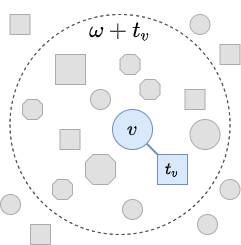
\includegraphics[width=0.42\columnwidth]{resources/ballroom/br2.png}
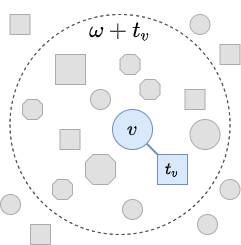
\includegraphics[width=0.21\columnwidth]{resources/ballroom/br2.png}
}\quad
\subfigure[]{
% 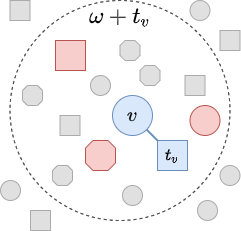
\includegraphics[width=0.42\columnwidth]{resources/ballroom/br3.png}
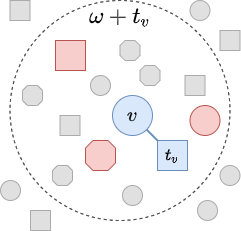
\includegraphics[width=0.21\columnwidth]{resources/ballroom/br3.png}
}\quad
\subfigure[]{
% 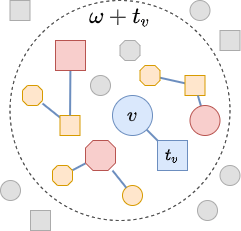
\includegraphics[width=0.42\columnwidth]{resources/ballroom/br4.png}
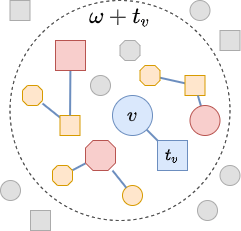
\includegraphics[width=0.21\columnwidth]{resources/ballroom/br4.png}
}\quad
\subfigure[]{
% 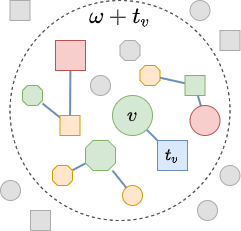
\includegraphics[width=0.42\columnwidth]{resources/ballroom/br5.png}
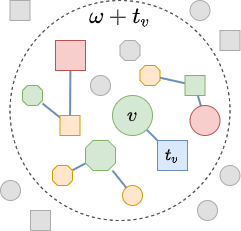
\includegraphics[width=0.21\columnwidth]{resources/ballroom/br5.png}
}\quad

\caption{
    Visual overview of Ballroom Walk temporal sampling algorithm.
    (a) The sampling timestamp $t_v$ for query node $v$ is inferred given the nearest neighbor if the node is static (blue). The relative time window is determined as $\omega + t_v$.
    (b) The root context nodes are sampled from the relative time window (red).
    (c) Context is extended with temporal random walks from the root nodes (yellow).
    (d) The context path is sampled from the collected context (green).
}
\label{fig:br}
\end{figure*}